%versi 3 (22-07-2020)
\chapter{Landasan Teori}
\label{chap:teori}
Pada bab ini, dibahas mengenai teori–teori yang digunakan dalam penelitian ini yaitu: \textit{CodeIgniter}, Dokumentasi SharIF-Judge, \textit{BASH}, \textit{JavaScript}, dan PHP

\section{\textit{JavaScript}}
\label{sec:JavaScript} 
Sementara HTML dan CSS membantu membuat desain halaman web, JavaScript membantu membuat fungsionalitas di halaman web \cite{javascriptlearn}. Java dan JavaScript memiliki nama yang sama tetapi keduanya merupakan bahasa pemrograman yang sangan berbeda.

%JavaScript merupakan bahasa pemrograman berorientasi objek berdasarkan model objek berbasis prototipe\cite{javascript_programming}.  Bahasa ini terkenal karena penggunaannya sebagai bahasa scripting di web. JavaScript dianggap sebagai blok pembangun utama HTML yang Dinamis dimana kumpulan teknologi yang disertakan pada hampir semua browser web dalam mendukung pembuatan situs web animasi dan interaktif. Saat terintegrasi di dalam browser web, implementasi JavaScript menyertakan sekumpulan pustaka yang secara kolektif disebut sebagai ``\textit{Client-Side JavaScript}'' Sebaliknya, bahasa JavaScript dan pustaka inti JavaScript (yaitu, pustaka yang mandiri dari web) biasanya disebut sebagai ``\textit{Core JavaScript}''% 

\subsection{Strings}
\label{sec: Strings}
    Pada JavaScript, String merupakan nilai yang terdiri dari teks dan dapat berisi huruf, angka, simbol, tanda baca, dan emoji\cite{javascriptlearn}. String \textit{JavaScript} terkandung dalam sepasang tanda kutip tunggal (') atau tanda kutip ganda (''). Kedua tanda kutip mewakili String tetapi pastikan untuk memilih salah satu. Jika dimulai dengan satu kutipan, maka harus diakhiri dengan satu kutipan. Sebagai contoh penulisannya adalah sebagai berikut:
    \begin{lstlisting}[basicstyle=\ttfamily, frame=single,
    columns=fullflexible, breaklines=true, numbers=none]
EXAMPLE
'This is a string.';
"This is the 2nd string.";
    \end{lstlisting}
    String tersebut tidak hanya untuk penulisan teks saja, namun ada berbagai fungsi logis yang dapat digunakan oleh pengguna yaitu sebagai berikut: 
    \begin{itemize}
        \item \textit{JavaScript String Length}\newline
        Tujuan fungsi logis ini adalah untuk menghitung panjang dari karater yang dituliskan. Contoh penulisannya adalah sebagai berikut: 
        \begin{lstlisting}[basicstyle=\ttfamily, frame=single,
        columns=fullflexible, breaklines=true, numbers=none]
EXAMPLE:
"caterpillar".length;
OUTPUT:
11
        \end{lstlisting}
        \item \textit{toLowerCase Method}\newline
        Fungsi logis \textit{toLowerCase} string dalam \textit{JavaScript} mengembalikan salinan string dengan huruf-hurufnya dikonversi menjadi huruf kecil. Namun untuk angka, simbol, dan karakter lain tidak terpengaruh dengan fungsi logis tersebut. Contoh penulisannya adalah sebagai berikut: 
         \begin{lstlisting}[basicstyle=\ttfamily, frame=single,
    columns=fullflexible, breaklines=true, numbers=none]
EXAMPLE:
"THE KIDS".toLowerCase();
OUTPUT:
"the kids"
        \end{lstlisting}
        \item \textit{toUpperCase Method}\newline
        Fungsi logis \textit{toUpperCase} string mengembalikan salinan string dengan huruf yang dikonversi menjadi huruf besar.Namun untuk angka, simbol, dan karakter lain tidak terpengaruh dengan fungsi logis tersebut. Contoh penulisannya adalah sebagai berikut: 
         \begin{lstlisting}[basicstyle=\ttfamily, frame=single,
    columns=fullflexible, breaklines=true, numbers=none]
EXAMPLE:
"I wish I were big.".toUpperCase();
OUTPUT:
"I WISH I WERE BIG."
        \end{lstlisting}
        \item \textit{trim}\newline
        Fungsi logis \textit{trim} string mengembalikan salinan string dengan karakter spasi awal dan akhir dihapus. Contoh penulisannya adalah sebagai berikut: 
        \begin{lstlisting}[basicstyle=\ttfamily, frame=single,
        columns=fullflexible, breaklines=true, numbers=none]
EXAMPLE:
"   but keep the middle spaces   ".trim();
OUTPUT:
"but keep the middle spaces"
        \end{lstlisting}
    \end{itemize}
    
\subsection{\textit{Numbers}}
\label{sec: Numbers}
   Bilangan adalah nilai yang dapat digunakan dalam operasi matematika\cite{javascriptlearn}. Untuk penulisan sintaks tidak diperlukan sesuatu yang khusus untuk angka dan cukup tuliskan langsung ke JavaScript. Contoh penulisannya adalah sebagai berikut: 
    \begin{lstlisting}[basicstyle=\ttfamily, frame=single,
    columns=fullflexible, breaklines=true, numbers=none]
EXAMPLE
12345;
    \end{lstlisting}
    \textit{Numbers} tersebut tidak hanya untuk penulisan angka saja, namun ada berbagai jenis yang dapat digunakan oleh pengguna yaitu sebagai berikut: 
    \begin{itemize}
        \item \textit{Decimals and fractions}\newline
        \textit{JavaScript} tidak membedakan antara bilangan bulat dan desimal, sehingga Anda dapat menggunakannya bersama-sama tanpa harus mengonversi dari satu ke yang lain. Contoh penulisannya adalah sebagai berikut: 
        \begin{lstlisting}[basicstyle=\ttfamily, frame=single,
        columns=fullflexible, breaklines=true, numbers=none]
EXAMPLE:
10 + 3.14159;
OUTPUT:
13.14159
        \end{lstlisting}
        \item \textit{Fractions}\newline
        Pecahan tidak ada dalam \textit{JavaScript}, tetapi dapat ditulis ulang sebagai masalah pembagian menggunakan operator pembagian ``/''. Perhatikan bahwa angka yang dihasilkan selalu dikonversi ke desimal sama seperti dengan kalkulator. Contoh penulisannya adalah sebagai berikut: 
        \begin{lstlisting}[basicstyle=\ttfamily, frame=single,
        columns=fullflexible, breaklines=true, numbers=none]
EXAMPLE:
1 / 3;
OUTPUT:
0.3333333333333333
        \end{lstlisting}
        Untuk menggunakan bilangan campuran, diperlukan penggabungan bilangan bulat dan pecahan. Contoh penulisannya adalah sebagai berikut: 
        \begin{lstlisting}[basicstyle=\ttfamily, frame=single,
    columns=fullflexible, breaklines=true, numbers=none]
EXAMPLE:
1 + (4 / 3);
OUTPUT:
2.333333333333333
        \end{lstlisting}
        \item \textit{Negative numbers}\newline
        Penulisan angka negatif dengan menempatkan operator di depan. Contoh penulisannya adalah sebagai berikut: 
        \begin{lstlisting}[basicstyle=\ttfamily, frame=single,
    columns=fullflexible, breaklines=true, numbers=none]
EXAMPLE:
-3;
OUTPUT:
-3;
        \end{lstlisting}
        Angka negatif dapat juga diperoleh dengan mengurangi angka dari angka yang lebih kecil. Contoh penulisannya adalah sebagai berikut: 
        \begin{lstlisting}[basicstyle=\ttfamily, frame=single,
    columns=fullflexible, breaklines=true, numbers=none]
EXAMPLE:
5-7;
OUTPUT:
-2;
        \end{lstlisting}
    \end{itemize}

\subsection{\textit{Booleans}}
\label{sec: Booleans}
    Dalam JavaScript, nilai boolean adalah nilai yang dapat berupa \textit{TRUE} atau \textit{FALSE}\cite{javascriptlearn}. Jika diperlukan mengetahui "ya" atau "tidak" tentang sesuatu, maka fungsi boolean merupakan fungsi yang tepat. Apa pun yang perlu "aktif" atau "mati", "ya" atau "tidak", "benar" atau "salah", atau yang hanya memiliki tujuan sementara, biasanya tepat untuk menggunakan boolean. Contoh penulisannya adalah sebagai berikut:
    \begin{lstlisting}[basicstyle=\ttfamily, frame=single,
    columns=fullflexible, breaklines=true, numbers=none]
EXAMPLE:
var kitchenLights = false;
kitchenLights = true;
kitchenLights;
OUTPUT:
true
        \end{lstlisting}
        Dalam contoh ini, variabel "kitchenLights" yang disetel ke "true" akan menunjukkan bahwa lampu menyala. Jika disetel ke "false" maka itu berarti mereka tidak aktif. Menyimpan boolean dalam variabel bertujuan untuk melacak nilainya dan mengubahnya dari waktu ke waktu. Boolean digunakan sebagai fungsi untuk mendapatkan nilai variabel, objek, kondisi, dan ekspresi. Faktanya, boolean sangat penting agar kondisional berfungsi.
        
\subsection{\textit{Operators}}
\label{sec: Operators}
   Operator adalah simbol antara nilai yang memungkinkan operasi yang berbeda seperti penambahan, pengurangan, perkalian, dan banyak lagi\cite{javascriptlearn}. Berikut ini merupakan operator yang dimiliki oleh \textit{javaScript}.
   \begin{itemize}
        \item \textit{Arithmetic}\newline
        Operator + menambahkan dua angka. Contoh penulisannya adalah sebagai berikut: 
        \begin{lstlisting}[basicstyle=\ttfamily, frame=single,
    columns=fullflexible, breaklines=true, numbers=none]
EXAMPLE:
1+2;
OUTPUT:
3
        \end{lstlisting}
        Operator - mengurangi satu angka dari angka lainnya. Contoh penulisannya adalah sebagai berikut: 
        \begin{lstlisting}[basicstyle=\ttfamily, frame=single,
    columns=fullflexible, breaklines=true, numbers=none]
EXAMPLE:
50 - 15;
OUTPUT:
35
        \end{lstlisting}
        Untuk menggunakan bilangan campuran, diperlukan penggabungan bilangan bulat dan pecahan. Contoh penulisannya adalah sebagai berikut:  
        \begin{lstlisting}[basicstyle=\ttfamily, frame=single,
    columns=fullflexible, breaklines=true, numbers=none]
EXAMPLE:
1 + (4 / 3);
OUTPUT:
2.333333333333333
        \end{lstlisting}
        Operator * mengalikan dua angka. Perhatikan bahwa itu adalah tanda bintang dan bukan simbol × yang biasa digunakan dalam matematika. Contoh penulisannya adalah sebagai berikut: 
        \begin{lstlisting}[basicstyle=\ttfamily, frame=single,
    columns=fullflexible, breaklines=true, numbers=none]
EXAMPLE:
3 * 12;
OUTPUT:
36
        \end{lstlisting}
        Operator / membagi satu nomor dengan yang lain. Perhatikan bahwa itu adalah garis miring dan bukan simbol yang biasa digunakan dalam matematika. Contoh penulisannya adalah sebagai berikut: 
        \begin{lstlisting}[basicstyle=\ttfamily, frame=single,
    columns=fullflexible, breaklines=true, numbers=none]
EXAMPLE:
12/4;
OUTPUT:
3;
        \end{lstlisting}
            Ekspresi JavaScript mengikuti urutan operasi, jadi meskipun + ditulis terlebih dahulu dalam contoh berikut, perkalian terjadi lebih dulu antara dua angka terakhir dan *. Contoh penulisannya adalah sebagai berikut: 
        \begin{lstlisting}[basicstyle=\ttfamily, frame=single,
    columns=fullflexible, breaklines=true, numbers=none]
EXAMPLE:
1 + 100 * 5;
OUTPUT:
501
        \end{lstlisting}
        \item \textit{Grouping} \newline
        () operator mengelompokkan nilai dan operasi lain. Kode yang terletak di antara tanda kurung dievaluasi terlebih dahulu saat JavaScript menyelesaikan setiap operasi yang bergerak dari kiri ke kanan. Menambahkan operator pengelompokan ke contoh sebelumnya menyebabkan 1 + 100 dievaluasi terlebih dahulu. Contoh penulisannya adalah sebagai berikut: 
        \begin{lstlisting}[basicstyle=\ttfamily, frame=single,
    columns=fullflexible, breaklines=true, numbers=none]
EXAMPLE:
(1 + 100) * 5;
OUTPUT:
505
        \end{lstlisting}
        \item \textit{Concatenation} \newline
        Operator + juga dapat menggabungkan string. Contoh penulisannya adalah sebagai berikut: 
        \begin{lstlisting}[basicstyle=\ttfamily, frame=single,
    columns=fullflexible, breaklines=true, numbers=none]
EXAMPLE:
"news" + "paper";
OUTPUT:
"newspaper"
        \end{lstlisting}
        \item \textit{Assignment} \newline
        Operator = memberikan nilai. Ini digunakan untuk mengatur nilai variabel. Contoh penulisannya adalah sebagai berikut: 
        \begin{lstlisting}[basicstyle=\ttfamily, frame=single,
    columns=fullflexible, breaklines=true, numbers=none]
EXAMPLE:
var dinner = "sushi";
        \end{lstlisting}
    \end{itemize}

\subsection{\textit{Variables}}
\label{sec: Variables}
   Variabel diberi nama nilai dan dapat menyimpan semua jenis nilai JavaScript\cite{javascriptlearn}. Contoh penulisannya adalah sebagai berikut: 
    \begin{lstlisting}[basicstyle=\ttfamily, frame=single,
    columns=fullflexible, breaklines=true, numbers=none]
EXAMPLE
var x = 100;
    \end{lstlisting}
    Penulisan diatas menyatakan hal sebagai berikut:
    \begin{itemize}
        \item var merupakan kata yang menyatakan kepada \textit{javascript} ingin mendeklarasikan sebuah variabel
        \item x adalah nama dari variabel yang dideklarasikan
        \item = merupakan operator yang menyatakan kepada \textit{javascript} bahwa kata selanjutnya adalah nilai dari variabel tersebut
        \item 100 adalah nilai dari variabel untuk disimpan
    \end{itemize}
    \begin{itemize}
        \item \textit{Using Variables}\newline
        Setelah mendeklarasikan variabel, variabel dapat direferensikan dengan nama di tempat lain dalam kode Anda. Contoh penulisannya adalah sebagai berikut: 
        \begin{lstlisting}[basicstyle=\ttfamily, frame=single,
    columns=fullflexible, breaklines=true, numbers=none]
EXAMPLE:
var x = 100;
x + 102;
OUTPUT:
202
        \end{lstlisting}
        nama variabel bahkan digunakan saat mendeklarasikan variabel lain.
        \begin{lstlisting}[basicstyle=\ttfamily, frame=single,
    columns=fullflexible, breaklines=true, numbers=none]
EXAMPLE:
var x = 100;
var y = x + 102;
y;
OUTPUT:
202
        \end{lstlisting}
        \item \textit{Reassigning variables}\newline
        Nilai baru dapat diberikan pada variabel yang ada kapan saja setelah dideklarasikan.
        
        \begin{lstlisting}[basicstyle=\ttfamily, frame=single,
        columns=fullflexible, breaklines=true, numbers=none]
EXAMPLE:
var weather = "rainy";
weather = "sunny";
weather;
OUTPUT:
"sunny"
        \end{lstlisting}

        \item \textit{Naming variables}\newline
        Penulisan nama variabel cukup fleksibel, namun ada beberapa aturan yang harus diikuti yaitu sebagai berikut: 
        \begin{itemize}
         \item Nama variabel harus diawali dengan huruf, garis bawah ``\_'', atau dolar ``\$''.
         \item Setelah huruf pertama, dapat digunakan angka, huruf, garis bawah, atau tanda dolar.
         \item Dilarang menggunakan kata kunci khusus dari \textit{JavaScript} apapun.
        \end{itemize}
        Maka dari itu berikut ini adalah contoh penulisan nama variabel yang valid 
         \begin{lstlisting}[basicstyle=\ttfamily, frame=single,
            columns=fullflexible, breaklines=true, numbers=none]
EXAMPLE:
var camelCase = "lowercase word, then uppercase";
var dinner2Go = "pizza";
var I_AM_HUNGRY = true;
var _Hello_ = "what a nice greeting"
var $_$ = "money eyes";
        \end{lstlisting}
    \end{itemize}
        --------------------------------------------------------------
\subsection{\textit{Functions}}
\label{sec: Functions}
   Fungsi \textit{JavaScript} adalah blok kode yang dapat digunakan kembali yang melakukan tugas tertentu, mengambil beberapa bentuk input dan mengembalikan output\cite{javascriptlearn}. Untuk mendefinisikan suatu fungsi, harus digunakan kata kunci fungsi, diikuti dengan nama, diikuti dengan tanda kurung ``( )''. Kemudian dituliskan logika fungsi di antara tanda kurung kurawal ``{}''. Contoh penulisannya adalah sebagai berikut: 
         \begin{lstlisting}[basicstyle=\ttfamily, frame=single,
            columns=fullflexible, breaklines=true, numbers=none]
EXAMPLE
function addTwoNumbers(x, y) {
    return x + y;
}
    \end{lstlisting}
    Setelah fungsi JavaScript didefinisikan atau dideklarasikan, fungsi dapat digunakan dengan merujuk namanya dengan tanda kurung tepat setelahnya. Perhatikan bahwa suatu fungsi tidak harus memiliki parameter.
         \begin{lstlisting}[basicstyle=\ttfamily, frame=single,
            columns=fullflexible, breaklines=true, numbers=none]
EXAMPLE:
function greetThePlanet() {
    return "Hello world!";
}
greetThePlanet();
OUTPUT:
"Hello world!"
    \end{lstlisting}
    Namun, jika suatu fungsi memiliki parameter, Anda harus memberikan nilai di dalam tanda kurung saat menggunakan fungsi:
         \begin{lstlisting}[basicstyle=\ttfamily, frame=single,
            columns=fullflexible, breaklines=true, numbers=none]
EXAMPLE:
function square(number) {
    return number * number;
}
square(16);
OUTPUT:
256
    \end{lstlisting}
    Dalam contoh di atas, \textit{number} tersebut harus diberikan angka agar fungsi berfungsi dan menerima output yang sesuai. Jika tidak, kode Anda tidak akan berfungsi dan Anda akan mendapatkan pesan kesalahan. Jika fungsi tersebut membutuhkan lebih dari satu argumen, pisahkan dengan menggunakan koma di dalam tanda kurung tersebut.
    
\subsection{\textit{Conditionals}}
\label{sec: Conditionals}
    \textit{Conditional statements} mengontrol perilaku dalam \textit{JavaScript} dan menentukan apakah potongan kode dapat dijalankan atau tidak\cite{javascriptlearn}. Terdapat 3 jenis kondisional dalam \textit{JavaScript} yaitu sebagai berikut: 
    \begin{itemize}
        \item \textit{IF}: di mana jika suatu kondisi benar, itu digunakan untuk menentukan eksekusi untuk blok kode.
        \item \textit{ELSE}: di mana jika kondisi yang sama salah, itu menentukan eksekusi untuk blok kode.
        \item \textit{ELSE IF}: ini menentukan tes baru jika kondisi pertama salah.
    \end{itemize}
    Berikut merupakan Contoh penulisan untuk \textit{IF}: 
    \begin{lstlisting}[basicstyle=\ttfamily, frame=single,
    columns=fullflexible, breaklines=true, numbers=none]
    EXAMPLE:
    if (10 > 5) {
    var outcome = "if block";
    }
    outcome;
    OUTPUT:
    "if block"
    \end{lstlisting}
    Berikut merupakan contoh penulisan untuk \textit{ELSE}
    \begin{lstlisting}[basicstyle=\ttfamily, frame=single,
    columns=fullflexible, breaklines=true, numbers=none]
    EXAMPLE:
if ("cat" === "dog") {
      var outcome = "if block";
} else {
      var outcome = "else block";
}
outcome;
    OUTPUT:
    "else block"
    \end{lstlisting}
    Berikut merupakan contoh penulisan untuk \textit{ELSE IF}
    \begin{lstlisting}[basicstyle=\ttfamily, frame=single,
    columns=fullflexible, breaklines=true, numbers=none]
    EXAMPLE:
    if (false) {
      var outcome = "if block";
    } else if (true) {
      var outcome = "else if block";
    } else {
      var outcome = "else block";
    }
    outcome;
    OUTPUT:
    "else if block"
    \end{lstlisting}

\subsection{\textit{Arrays}}
\label{sec: Arrays}
Array adalah nilai seperti wadah yang dapat menampung nilai lain\cite{javascriptlearn}. Nilai-nilai di dalam array disebut elemen. Contoh penulisannya sebagai berikut: 
    \begin{lstlisting}[basicstyle=\ttfamily, frame=single,
    columns=fullflexible, breaklines=true, numbers=none]
    EXAMPLE:
    var breakfast = ["coffee", "croissant"];
    breakfast;
    OUTPUT:
    ["coffee", "croissant"]
    \end{lstlisting}
    Elemen pada array tidak semuanya harus memiliki tipe nilai yang sama. Elemen dapat berupa nilai JavaScript apa pun bahkan array lainnya. Contohnya penulisannya sebagai berikut: 
        \begin{lstlisting}[basicstyle=\ttfamily, frame=single,
    columns=fullflexible, breaklines=true, numbers=none]
    EXAMPLE:
    var hodgepodge = [100, "paint", [200, "brush"], false];
    hodgepodge;
    OUTPUT:
    [100, "paint", [200, "brush"], false]
    \end{lstlisting}
    Untuk mengakses salah satu elemen di dalam array, harus digunakan tanda kurung dan angka seperti ini: myArray[3]. Array JavaScript dimulai dari 0, jadi elemen pertama akan selalu berada di dalam [0].
    \begin{lstlisting}[basicstyle=\ttfamily, frame=single,
    columns=fullflexible, breaklines=true, numbers=none]
    EXAMPLE:
    var sisters = ["Tia", "Tamera"];
    sisters[0];
    OUTPUT:
    "Tia"
    \end{lstlisting}
    Untuk mendapatkan elemen terakhir, Anda dapat menggunakan tanda kurung dan `1` kurang dari properti panjang larik.
    \begin{lstlisting}[basicstyle=\ttfamily, frame=single,
    columns=fullflexible, breaklines=true, numbers=none]
    EXAMPLE:
    var actors = ["Felicia", "Nathan", "Neil"];
    actors[actors.length - 1];
    OUTPUT:
    "Neil"
    \end{lstlisting}
    
\subsection{\textit{Objects}}
\label{sec: Objects}
Objek pada JavaScript adalah variabel yang berisi beberapa nilai data. Nilai dalam objek JavaScript dikenal sebagai properti\cite{javascriptlearn}. Objek menggunakan kunci untuk menamai nilai, seperti yang dilakukan dengan variabel. Contohnya adalah sebagai berikut: 
    \begin{lstlisting}[basicstyle=\ttfamily, frame=single,
    columns=fullflexible, breaklines=true, numbers=none]
    EXAMPLE:
    var course = {
       name: "GRA 2032",
       start: 8,
       end: 10
    };
    \end{lstlisting}
    Ada dua cara untuk mengakses nilai properti objek. Dapat digunakan notasi titik dengan nama properti setelah titik objectName.propertyName seperti pada contoh di bawah ini:
    \begin{lstlisting}[basicstyle=\ttfamily, frame=single,
    columns=fullflexible, breaklines=true, numbers=none]
    EXAMPLE:
    var course = {
       name: "GRA 2032",
       start: 8,
       end: 10
    };
    course.name;
    OUTPUT:
    "GRA 2032"
    \end{lstlisting}
    Atau Dapat digunakan notasi braket dengan nama properti di dalam string di dalam tanda kurung siku - objectName[“propertyName”] seperti pada contoh di bawah ini:
    \begin{lstlisting}[basicstyle=\ttfamily, frame=single,
    columns=fullflexible, breaklines=true, numbers=none]
    EXAMPLE:
    var course = {
       name: "GRA 2032",
       start: 8,
       end: 10
    };
    course["name"];
    OUTPUT:
    "GRA 2032"
    \end{lstlisting}
    
\section{CodeIgniter 3}
\label{sec:CodeIgniter} 
 
CodeIgniter merupakan sebuah \textit{framework} bagi pengguna yang ingin membangun \textit{web application} dengan menggunakan bahasa pemrograman berbasis PHP\cite{codeigniter}. Tujuan utamanya adalah untuk mempercepat pengerjaan para pengguna agar tidak perlu menuliskan kode dari awal. Dengan menyediakan kumpulan \textit{libraries} yang kaya untuk tugas-tugas umum yang dibutuhkan, serta antarmuka sederhana dan struktur logis untuk mengakses pustaka ini. SharIF-Judge menggunakan CodeIgniter 3. Untuk dapat menggunakan CodeIgniter 3 direkomendasikan PHP versi 5.6 atau yang lebih baru dari itu dengan alasan agar tidak memiliki permasalahan terhadap bagian keamanan, permasalahan perfoma, dan adanya fitur yang hilang. Database yang dapat didukung oleh CodeIgniter 3 adalah sebagai berikut:
\begin{itemize}
    \item MySQL (5.1+) via the mysql (deprecated), mysqli and pdo drivers
    \item Oracle via the oci8 and pdo drivers
    \item PostgreSQL via the postgre and pdo drivers
    \item MS SQL via the mssql, sqlsrv (version 2005 and above only) and pdo drivers
    \item SQLite via the sqlite (version 2), sqlite3 (version 3) and pdo drivers
    \item CUBRID via cubrid dan pdo \textit{drivers}
    \item Interbase/Firebird via ibase dan pdo \textit{drivers}
    \item ODBC via the odbc dan pdo \textit{drivers} 
\end{itemize}

\subsection{\textit{Application Flow Chart}}
\label{sec: Application Flow Chart}

Gambar \ref{fig:flowchart} merupakan ilustrasi bagaimana data mengalir ke seluruh sistem\cite{codeigniter}.
 \begin{figure}[h!]
     \centering
     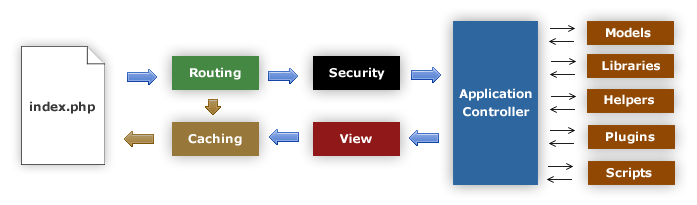
\includegraphics[width=0.9\linewidth]{Gambar/appflowchart.png}
     \caption{\textit{Flow Chart}Aplikasi}
     \label{fig:flowchart}
 \end{figure}
 
Berikut ini merupakan penjelasan secara urut dari awal sampai akhir bagaimana sistem mengalir:
\begin{enumerate}
    \item \textit{File} \textit{index.php} berfungsi sebagai pengontrol depan, menginisialisasi sumber daya dasar yang diperlukan untuk menjalankan CodeIgniter.
    \item Router memeriksa permintaan HTTP untuk menentukan apa yang harus dilakukan.
    \item Jika terdapat \textit{file cache}, maka akan langsung dikirimkan ke \textit{browser}. \textit{File cache} adalah data yang pernah diakses oleh pengguna. Data tersebut dapat berupa teks, gambar atau file.
    \item \textit{HTTP request} dan data pengguna yang dikirim akan disaring terlebih dahulu untuk keamanan. \textit{Application controller} akan dimuat setelah proses penyaringan selesai.
    \item \textit{Controller} akan memuat kelas Model, \textit{library} utama dan kelas bantuan.
    \item \textit{View} akan memuat tampilan akhir dan dikirim ke \textit{web browser}. Jika \textit{caching} diaktifkan, maka tampilan dimasukan ke dalam \textit{cache} terlebih dahulu sehingga pada permintaan selanjutnya tampilan tersebut dapat diakses lebih cepat.
\end{enumerate}

\subsection{\textit{Model-View-Controller}}
\label{sec:Model-View-Controller}
CodeIgniter didasarkan pada pola pengembangan Model-View-Controller\cite{codeigniter}. MVC adalah pendekatan perangkat lunak yang memisahkan logika aplikasi dari presentasi. Dalam praktiknya, ini memungkinkan halaman web Anda berisi skrip minimal karena presentasinya terpisah dari skrip PHP.  MVC merupakan kumpulan dari tiga bagian: Model, View, dan Controller. 

 \begin{figure}[h!]
     \centering
     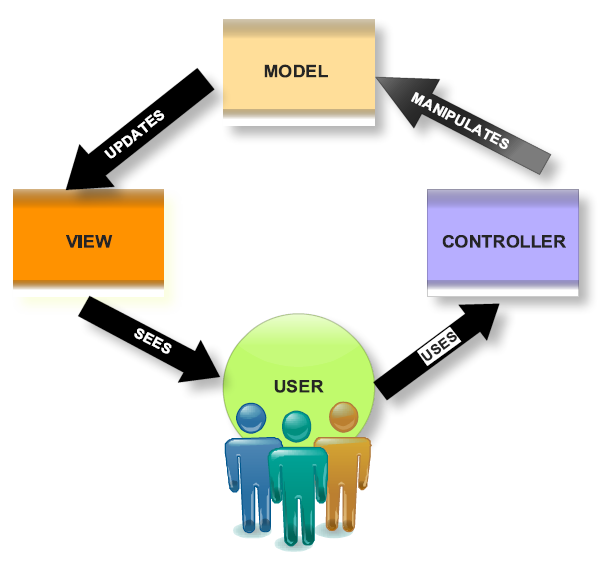
\includegraphics[width=0.5\linewidth]{Gambar/MVC.PNG}
     \caption{Perputaran \textit{Model-View-Controller}}
     \label{fig:label}
 \end{figure}
Gambar \ref{fig:label} menunjukkan pola dan interaksi dengan pengguna dan aplikasi itu sendiri. Ini adalah tata letak aliran tunggal data, bagaimana data itu dilewatkan di antara setiap komponen, dan akhirnya bagaimana hubungan antara setiap komponen bekerja. 


\subsubsection{\textit{Model}}
\label{sec:Model}
Model adalah kelas PHP yang dirancang untuk bekerja dengan informasi dalam database\cite{codeigniter}. Berikut adalah contoh tampilan kelas \textit{model}:
\begin{lstlisting}[basicstyle=\ttfamily, frame=single,
    columns=fullflexible, breaklines=true, numbers=none]
class Blog_model extends CI_Model {

        public $title;
        public $content;
        public $date;

        public function get_last_ten_entries()
        {
                $query = $this->db->get('entries', 10);
                return $query->result();
        }

        public function insert_entry()
        {
                $this->title    = $_POST['title']; // please read the below note
                $this->content  = $_POST['content'];
                $this->date     = time();

                $this->db->insert('entries', $this);
        }

        public function update_entry()
        {
                $this->title    = $_POST['title'];
                $this->content  = $_POST['content'];
                $this->date     = time();

                $this->db->update('entries', $this, array('id' => $_POST['id']));
        }

}
    \end{lstlisting}
    model biasanya akan dimuat dan dipanggil dari dalam \textit{control}. Untuk memuat model, dapat digunakan metode berikut:
    \begin{lstlisting}[basicstyle=\ttfamily, frame=single,
    columns=fullflexible, breaklines=true, numbers=none]
$this->load->model('model_name');
    \end{lstlisting}
    jika model terletak di sub-direktori, sertakan jalur relatif dari direktori model. Misalnya, jika memiliki model yang terletak di application/models/blog/Queries.php, dapat dimuat menggunakan:
    \begin{lstlisting}[basicstyle=\ttfamily, frame=single,
    columns=fullflexible, breaklines=true, numbers=none]
$this->load->model('blog/queries');
    \end{lstlisting}
    Ketika sebuah model dimuat itu tidak terhubung secara otomatis ke database. Berikut merupakan opsi alternatif untuk menghubungkan:
    \begin{itemize}
        \item Terhubung menggunakan metode database standar yang dijelaskan pada dokumentasi, baik dari dalam kelas \textit{Controller} atau kelas \textit{Model}.
        \item Memberi tahu metode pemuatan \textit{model} untuk terhubung secara otomatis dengan meneruskan \textit{TRUE} (boolean) melalui parameter ketiga, dan pengaturan konektivitas, seperti yang ditentukan dalam \textit{file} konfigurasi database yang akan digunakan, berikut cara menuliskannya: 
        \begin{lstlisting}[basicstyle=\ttfamily, frame=single,
        columns=fullflexible, breaklines=true, numbers=none]
$this->load->model('model_name', '', TRUE);
    \end{lstlisting}
    \item melewati pengaturan konektivitas basis data secara manual melalui parameter ketiga:
    \begin{lstlisting}[basicstyle=\ttfamily, frame=single,
        columns=fullflexible, breaklines=true, numbers=none]
$config['hostname'] = 'localhost';
$config['username'] = 'myusername';
$config['password'] = 'mypassword';
$config['database'] = 'mydatabase';
$config['dbdriver'] = 'mysqli';
$config['dbprefix'] = '';
$config['pconnect'] = FALSE;
$config['db_debug'] = TRUE;

$this->load->model('model_name', '', $config);
    \end{lstlisting}
    \end{itemize}
\subsubsection{\textit{View}}
\label{sec:View} 
\textit{View} tidak pernah dipanggil secara langsung, \textit{view} harus dimuat oleh \textit{controller}. Dalam kerangka MVC, Controller bertindak sebagai polisi lalu lintas, sehingga bertanggung jawab untuk mengambil tampilan tertentu. berikut merupakan contoh kode program pada file \textit{view}: 
    \begin{lstlisting}[basicstyle=\ttfamily, frame=single,
        columns=fullflexible, breaklines=true, numbers=none]
<html>
<head>
        <title>My Blog</title>
</head>
<body>
        <h1>Welcome to my Blog!</h1>
</body>
</html>
    \end{lstlisting}
    Untuk memuat file tampilan tertentu, dapat digunakan metode berikut:
    \begin{lstlisting}[basicstyle=\ttfamily, frame=single,
        columns=fullflexible, breaklines=true, numbers=none]
$this->load->view('name');
    \end{lstlisting}    
    Jika lebih dari satu panggilan terjadi \textit{view} akan ditambahkan bersama-sama. Misalnya, ingin dimiliki tampilan header, tampilan menu, tampilan konten, dan tampilan footer. akan terlihat sebagai berikut:
    \begin{lstlisting}[basicstyle=\ttfamily, frame=single,
        columns=fullflexible, breaklines=true, numbers=none]
<?php

class Page extends CI_Controller {

        public function index()
        {
                $data['page_title'] = 'Your title';
                $this->load->view('header');
                $this->load->view('menu');
                $this->load->view('content', $data);
                $this->load->view('footer');
        }

}
    \end{lstlisting}    
    \textit{File} juga dapat disimpan dalam sub-direktori saat melakukannya, harus disertakan nama direktori yang memuat tampilan. Contoh:
    \begin{lstlisting}[basicstyle=\ttfamily, frame=single,
        columns=fullflexible, breaklines=true, numbers=none]
$this->load->view('directory_name/file_name');
    \end{lstlisting}  
\textit{View} juga dapat mengeluarkan tampilan lebih dari satu dengan menggunakan array. Berikut adalah contoh sederhana. Tambahkan ini ke \textit{Controller}:
    \begin{lstlisting}[basicstyle=\ttfamily, frame=single,
        columns=fullflexible, breaklines=true, numbers=none]
<?php
class Blog extends CI_Controller {

        public function index()
        {
                $data['todo_list'] = array('Clean House', 'Call Mom', 'Run Errands');

                $data['title'] = "My Real Title";
                $data['heading'] = "My Real Heading";

                $this->load->view('blogview', $data);
        }
}
    \end{lstlisting}  
    lalu pada \textit{View} buatlah kode seperti ini:
     \begin{lstlisting}[basicstyle=\ttfamily, frame=single,
        columns=fullflexible, breaklines=true, numbers=none]
<html>
<head>
        <title><?php echo $title;?></title>
</head>
<body>
        <h1><?php echo $heading;?></h1>

        <h3>My Todo List</h3>

        <ul>
        <?php foreach ($todo_list as $item):?>

                <li><?php echo $item;?></li>

        <?php endforeach;?>
        </ul>

</body>
</html>
    \end{lstlisting}    
    
\subsubsection{\textit{Controller}}
\label{sec:Controller} 
Komponen ketiga dari MVC adalah \textit{Controller}. Tugasnya adalah menangani data yang dikirimkan pengguna serta memperbarui \textit{Model} yang sesuai \cite{codeigniter}. CodeIgniter dapat diminta untuk memuat \textit{controller} \textit{default} ketika URI tidak ada, seperti halnya ketika hanya URL root situs yang diminta. Untuk menentukan pengontrol default, buka file application/config/routes.php dan atur variabel ini:

     \begin{lstlisting}[basicstyle=\ttfamily, frame=single,
        columns=fullflexible, breaklines=true, numbers=none]
$route['default_controller'] = 'blog';
    \end{lstlisting} 

'blog' adalah nama kelas \textit{controller} yang ingin digunakan. Jika sekarang dimuat file index.php utama tanpa menentukan segmen URI apa pun, akan terlihat pesan "Hello World" secara default. CodeIgniter memiliki kelas keluaran yang menangani pengiriman data akhir ke \textit{browser web} secara otomatis. Informasi lebih lanjut tentang ini dapat ditemukan di halaman \textit{View} dan kelas \textit{Output}. CodeIgniter mengizinkan penambahan metode bernama \_output() ke \textit{controller} yang akan menerima data keluaran akhir. Contohnya sebagai berikut: 

     \begin{lstlisting}[basicstyle=\ttfamily, frame=single,
        columns=fullflexible, breaklines=true, numbers=none]
public function _output($output)
{
        echo $output;
}
    \end{lstlisting} 

\section{BASH}
\label{sec:BASH}
BASH adalah penerjemah default pada banyak sistem GNU/Linux yang merupakan singkatan dari \textit{Bourne Again SHell}, Bash adalah  shell yang kompatibel yang menggabungkan fitur berguna dari \textit{Korn shell} (ksh) dan \textit{C Shell}(csh)\cite{gnu}. BASH menawarkan peningkatan fungsional atas sh untuk pemrograman dan penggunaan interaktif. Selain itu, sebagian besar skrip shell dapat dijalankan oleh Bash tanpa modifikasi. Kelebihan yang dapat diberikan oleh Bash antara lain sebagai berikut
\begin{itemize}
    \item Edit pada \textit{command-line}
    \item Riwayat penulisan perintah yang tidak dibatasi
    \item Kontrol pekerjaan
    \item Fungsi dari shell
    \item array dengan index tidak terbatas
    \item bilangan integer dari hanya 2 bit sampai 64 bit
\end{itemize}

\section{Node.js}
\label{sec: Node.js}
Node.js adalah lingkungan runtime JavaScript \textit{open-source} dan lintas platform\cite{nodejs}. Ini adalah alat yang populer untuk hampir semua jenis proyek Node.js menjalankan \textit{engine} JavaScript V8, inti dari Google Chrome, di luar browser. Ini memungkinkan Node.js menjadi sangat berkinerja.

Aplikasi Node.js berjalan dalam satu proses, tanpa membuat thread baru untuk setiap permintaan.
Saat Node.js melakukan operasi \textit{Input}/\textit{Output} (I/O), seperti membaca dari jaringan, mengakses database atau sistem file, alih-alih memblokir \textit{thread} dan membuang siklus CPU menunggu, Node.js akan melanjutkan operasi saat respons kembali.

Hal ini memungkinkan Node.js untuk menangani ribuan koneksi bersamaan dengan satu server tanpa menimbulkan beban mengelola konkurensi \textit{thread}, yang dapat menjadi sumber \textit{bug} yang signifikan.

Di Node.js, standar ECMAScript baru dapat digunakan tanpa masalah, karena tidak perlu menunggu semua pengguna memperbarui browser user dan bertanggung jawab untuk memutuskan versi ECMAScript mana yang akan digunakan dengan mengubah versi Node.js, dan juga dapat mengaktifkan fitur eksperimental tertentu dengan menjalankan Node.js dengan \textit{flag}.

\subsection{\textit{Twig}}
Pada perangkat lunak SharIF-Judge, kelas \textit{view} menggunakan \textit{framework} aplikasi yaitu \textit{Twig}. \textit{Twig} merupakan sebuah \textit{template engine modern} untuk PHP\cite{twig}. Sebuah \textit{template} \textit{Twig} dapat mengandung variables atau \textit{expression} dan \textit{tags}. \textit{Variables} atau \textit{expression} akan diubah pada saat \textit{template} \textit{Twig} dievaluasi dan \textit{tags} yang akan mengontrol logika dari \textit{template} tersebut. Berikut merupakan \textit{template} kode yang menunjukan beberapa hal mendasar.

 \begin{lstlisting}[basicstyle=\ttfamily, frame=single,
    columns=fullflexible, breaklines=true, numbers=none]
<!DOCTYPE html>
<html>
    <head>
        <title>My Webpage</title>
    </head>
    <body>
        <ul id="navigation">
        
        <li><a href="{{ item.href }}">{{ item.caption }}</a></li>
        
        </ul>
        <h1>My Webpage</h1>
        {{ a_variable }}
    </body>
</html>
    \end{lstlisting}

Ada dua jenis delimiters pada kode di atas, yaitu {\% ... \%} dan {{ ... }}. \textit{Delimiters} {\% ... \%} digunakan untuk mengeksekusi sebuah \textit{statements}. Pada kode di atas, \textit{delimiters} {\% for item in navigation \%} akan mengeksekusi \textit{statements for-loops} atau pengulangan. \textit{Delimiters} {{ ... }} digunakan untuk menampilkan nilai. Pada kode di atas, \textit{delimiters} {{ item.href }} akan menampilkan nilai item.href, \textit{delimiters} {{ item.caption }} akan menampilkan nilai item.caption dan \textit{delimiters} {{ a\_variable }} akan menampilkan nilai a\_variable.




%https://codeigniter.com/userguide3/general/requirements.html
